\section{The notion of limit} \label{S:1.1.Limits}

\begin{goals}
\item What is the behavior of a function arbitrarily close to, but not necessarily at, a specific point?
\item What is the mathematical notion of \emph{limit} and what role do limits play in the study of functions?
\item What is the meaning of the notation $\ds \lim_{x \to a} f(x) = L$?
\item How do we go about determining the value of the limit of a function at a point?
\item How does the notion of limit allow us to move from average velocity to instantaneous velocity?
\end{goals}

%-----------------------------------
% SUBSECTION INTRODUCTION
%-----------------------------------
\subsection*{Introduction}

Functions are at the heart of mathematics: a function is a process or rule that associates each individual input to exactly one corresponding output.  Students learn in courses prior to calculus that there are many different ways to represent functions, including through formulas, graphs, tables, and even words.  For example, the squaring function can be thought of in any of these ways.  In words, the squaring function takes any real number $x$ and computes its square.  The formulaic and graphical representations go hand in hand, as $y = f(x) = x^2$ is one of the simplest curves to graph.  Finally, we can also partially represent this function through a table of values, essentially by listing some of the ordered pairs that lie on the curve, such as  $(-2,4)$, $(-1,1)$, $(0,0)$, $(1,1)$, and $(2,4)$.

Functions are especially important in calculus because they often model important phenomena -- the location of a moving object at a given time, the rate at which an automobile is consuming gasoline at a certain velocity, the reaction of a patient to the size of a dose of a drug -- and calculus can be used to study how these output quantities change in response to changes in the input variable.  Moreover, thinking about concepts like average and instantaneous velocity leads us naturally from an initial function to a related, sometimes more complicated function.  As one example of this, think about the falling ball whose position function is given by $s(t) = 64 - 16t^2$ and the average velocity of the ball on the interval $[1,x]$.  Observe that
\[ AV_{[1,x]} = \frac{s(x) - s(1)}{x-1} = \frac{(64-16x^2) - (64-16)}{x-1} = \frac{16 - 16x^2}{x-1}. \]
Now, two things are essential to note:  this average velocity depends on $x$ (indeed, $AV_{[1,x]}$ is a function of $x$), and our most focused interest in this function occurs near $x = 1$, which is where the function is not defined.  Said differently, the function $g(x) = \frac{16 - 16x^2}{x-1}$ tells us the average velocity of the ball on the interval from $t = 1$ to $t = x$, and if we are interested in the instantaneous velocity of the ball when $t = 1$, we'd like to know what happens to $g(x)$ as $x$ gets closer and closer to $1$.  At the same time, $g(1)$ is not defined, because it leads to the quotient $0/0$.

This is where the idea of \emph{limits} comes in.  By using a limit, we'll be able to allow $x$ to get arbitrarily close, but not equal, to $1$ and fully understand the behavior of $g(x)$ near this value.  We'll develop key language, notation, and conceptual understanding in what follows, but for now we consider a preliminary activity that uses the graphical interpretation of a function to explore points on a graph where interesting behavior occurs.

\begin{marginfigure}[8cm]
\margingraphics{figures/1_2_PA1.eps} 
\caption{Graph of $y = g(x)$ for Preview Activity~\ref{PA:1.1}.} \label{fig:1.1.PA1}
\end{marginfigure}

\begin{pa} \label{PA:1.1}
Suppose that $g$ is the function given by the Figure~\ref{fig:1.1.PA1}.  Use the graph to answer each of the following questions. 
\ba
	\item Determine the values $g(-2)$, $g(-1)$, $g(0)$, $g(1)$, and $g(2)$, if defined.  If the function value is not defined, explain what feature of the graph tells you this.
	\item For each of the values $a = -1$, $a = 0$, and $a = 2$, complete the following sentence: ``As $x$ gets closer and closer (but not equal) to $a$, $g(x)$ gets as close as we want to \underline{\hspace{0.3in}}.''
	\item What happens as $x$ gets closer and closer (but not equal) to $a = 1$?  Does the function $g(x)$ get as close as we would like to a single value?
\ea

\end{pa} \afterpa %ACTIVITY

%-----------------------------------------------------------------
% SUBSECTION THE AVERAGE VALUE OF A FUNCTION
%-----------------------------------------------------------------
\subsection*{The Idea of a Limit}

Limits can be thought of as a way to study the tendency or trend of a function as the input variable approaches a fixed value, or even as the input variable increases or decreases without bound.  Here, we focus on what it means to say that ``a function $f$ has limit $L$ as $x$ approaches $a$.''  To begin, we think about a recent example.

In Preview Activity \ref{PA:1.1}, you saw that for the given function $g$, as $x$ gets closer and closer (but not equal) to $0$, $g(x)$ gets as close as we want to the value $4$.  At first, this may feel counterintuitive, because the value of $g(0)$ is $1$, not $4$.  By their very definition, limits regard the behavior of a function \emph{arbitrarily close to} a fixed input, but the value of the function \emph{at} the fixed input does not matter.  More formally\footnote{What follows here is not what mathematicians consider the formal definition of a limit.  To be completely precise, it is necessary to quantify both what it means to say ``as close to $L$ as we like'' and ``sufficiently close to $a$.''  That can be accomplished through what is traditionally called the epsilon-delta definition of limits, which will be covered in Section \ref{S:1.4.precise}.}, we say the following.

\definition{The Limit of a Function}{ %DEFINITION
Given a function $f$, a fixed input $x = a$, and a real number $L$, we say that \emph{$f$ has limit\index{limit!definition} $L$ as $x$ approaches $a$}, and write
\[ \lim_{x \to a} f(x) = L \]
provided that we can make $f(x)$ as close to $L$ as we like by taking $x$ sufficiently close (but not equal) to $a$.  If we cannot make $f(x)$ as close to a single value as we would like as $x$ approaches $a$, then we say that \emph{$f$ does not have a limit as $x$ approaches $a$.}
} % end definition

For the function $g$ pictured in Figure \ref{fig:1.1.PA1}, we can make the following observations:  
\[ \ds \lim_{x \to -1} g(x) = 3, \ \ds \lim_{x \to 0} g(x) = 4, \ \mbox{and} \ \ds \lim_{x \to 2} g(x) = 1, \] 
but $g$ does not have a limit as $x \to 1$.  When working graphically, it suffices to ask if the function approaches a single value from each side of the fixed input, while understanding that the function value right at the fixed input is irrelevant.  This reasoning explains the values of the first three stated limits.  In a situation such as the jump in the graph of $g$ at $x = 1$, the issue is that if we approach $x = 1$ from the left, the function values tend to get as close to $3$ as we'd like, but if we approach $x = 1$ from the right, the function values get as close to $2$ as we'd like, and there is no single number that all of these function values approach.  This is why the limit of $g$ does not exist at $x = 1$.

For any function $f$, there are typically three ways to answer the question ``does $f$ have a limit at $x = a$, and if so, what is the limit?''  The first is to reason graphically as we have just done with the example from Preview Activity \ref{PA:1.1}.  If we have a formula for $f(x)$, there are two additional possibilities:  (1) evaluate the function at a sequence of inputs that approach $a$ on either side, typically using some sort of computing technology, and ask if the sequence of outputs seems to approach a single value; (2) use the algebraic form of the function to understand the trend in its output as the input values approach $a$.  The first approach only produces an approximation of the value of the limit, while the latter can often be used to determine the limit exactly.  The following examples demonstrate the  approaches of using a table and graph to evaluate limits.

\begin{margintable}
\scalebox{1.1}{
\begin{tabular}{cc}
	\raisebox{-.5in}{
	\begin{tabular}[b]{r|l} 
	$x$ & $f(x)$ \\ 
	\hline $-0.9$ & $2.9$ \\ 
	$-0.99$ & $2.99$ \\ 
	$-0.999$ & $2.999$ \\ 
	$-0.9999$ & $2.9999$ \\ 
	$-1.1$ & $3.1$ \\ 
	$-1.01$ & $3.01$ \\ 
	$-1.001$ & $3.001$ \\ 
	$-1.0001$ & $3.0001$ \\ 
	\end{tabular} } &	
	\raisebox{-.5in}{
	\begin{tabular}[b]{r|l} 
	$x$ & $f(x)$ \\ 
	\hline $-1.9$ & $3.9$ \\ 
	$-1.99$ & $3.99$ \\ 
	$-1.999$ & $3.999$ \\ 
	$-1.9999$ & $3.9999$ \\ 
	$-2.1$ & $4.1$ \\ 
	$-2.01$ & $4.01$ \\ 
	$-2.001$ & $4.001$ \\ 
	$-2.0001$ & $4.0001$ \\ 
	\end{tabular} }
\end{tabular}
} % end scalebox 
\caption{Function values near $-1$ and $-2$.} \label{T:1-1_Eg1}
\end{margintable}

\begin{marginfigure}
\margingraphics{figures/1_2_Ex1f.eps}
\caption{The graph of $f(x) = \frac{4-x^2}{x+2}$ near $-1$ and $-2$.}\label{fig:1-1_Eg1}
\end{marginfigure}

\begin{example} \label{Ex:1.1.Eg1}
Use both tables and graphical approaches to investigate and, if possible, estimate or determine the value of the limit for the following function at the specified values.  
\[ \ds f(x) = \frac{4-x^2}{x+2}; \quad a = -1, \ a = -2 \]

\solution We first construct tables of values near $a = -1$ and $a = -2$, see Table~\ref{T:1-1_Eg1}, along with a graph of $f$, see Figure~\ref{fig:1-1_Eg1}.  

From the left table, it appears that we can make $f$ as close as we want to $3$ by taking $x$ sufficiently close to $-1$, which suggests that $\ds \lim_{x \to -1} f(x) = 3$.	This is also consistent with the graph of $f$.  

From the right table, it appears that we can make $f$ as close as we want to $4$ by taking $x$ sufficiently close, but not equal since $f(-2)$ is not defined, to $-2$, which suggests that $\ds \lim_{x \to -4} f(x) = 4$.	Remember, limits ask, ``To where is the function going?'', not ``What is the value of the function?''  Again, this observation is  consistent with the graph of $f$.  

%Next we turn to the function $g$, and construct two tables and a graph.
%\begin{figure}[h]
%\centering
%\begin{tabular}{ccc}
%	\raisebox{-.05in}{\begin{tabular}[b]{r|l} $x$ & $g(x)$ \\ \hline 2.9 & 0.84864 \\ 2.99 & 0.86428 \\ 2.999 & 0.86585 \\ 2.9999 & 0.86601 \\ 3.1 & 0.88351 \\ 3.01 &  0.86777 \\ 3.001 & 0.86620 \\ 3.0001 &  0.86604 \\ \end{tabular} } &	
%	\raisebox{-.05in}{\begin{tabular}[b]{r|l} $x$ & $g(x)$ \\ \hline -0.1 & 0 \\ -0.01 & 0 \\ -0.001 & 0 \\ -0.0001 & 0 \\ 0.1 & 0 \\ 0.01 & 0 \\ 0.001 & 0 \\ 0.0001 & 0 \\ \end{tabular} } &
%	\hspace{0.25in} 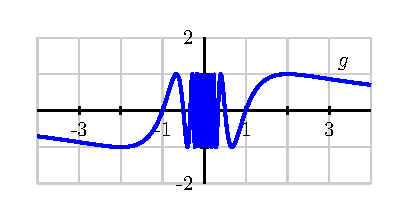
\includegraphics{figures/1_2_Ex1g.eps} 
%\end{tabular}
%\caption{Tables and graph for $\ds g(x) = \sin\left(\frac{\pi}{x}\right)$.} \label{F:1.2.Ex1g}
%\end{figure}

%First, as $x \to 3$, it appears from the data (and the graph) that the function is approaching approximately $0.866025$.  To be precise, we have to use the fact that $\frac{\pi}{x} \to \frac{\pi}{3}$, and thus we find that $g(x) = \sin(\frac{\pi}{x}) \to \sin(\frac{\pi}{3})$ as $x \to 3$.  The exact value of $\sin(\frac{\pi}{3})$ is $\frac{\sqrt{3}}{2}$, which is approximately 0.8660254038.  Thus, we see that
%$$\lim_{x \to 3} g(x) = \frac{\sqrt{3}}{2}.$$
%
%As $x \to 0$, we observe that $\frac{\pi}{x}$ does not behave in an elementary way.  When $x$ is positive and approaching zero, we are dividing by smaller and smaller positive values, and $\frac{\pi}{x}$ increases without bound.  When $x$ is negative and approaching zero, $\frac{\pi}{x}$ decreases without bound.  In this sense, as we get close to $x = 0$, the inputs to the sine function are growing rapidly, and this leads to wild oscillations in the graph of $g$.  It is an instructive exercise to plot the function $g(x) = \sin\left(\frac{\pi}{x}\right)$ with a graphing utility and then zoom in on $x = 0$.  Doing so shows that the function never settles down to a single value near the origin and suggests that $g$ does not have a limit at $x = 0$.

\end{example} % EXAMPLE

\begin{margintable}
\scalebox{1.15}{
\begin{tabular}{cc}
	\raisebox{-.05in}{
	\begin{tabular}[b]{r|l} 
	$x$ & $g(x)$ \\ 
	\hline 2.9 & 0.84864 \\ 
	2.99 & 0.86428 \\ 
	2.999 & 0.86585 \\ 
	2.9999 & 0.86601 \\ 
	3.1 & 0.88351 \\ 
	3.01 &  0.86777 \\ 
	3.001 & 0.86620 \\ 
	3.0001 &  0.86604 \\ 
	\end{tabular} } &	
	\raisebox{-.05in}{
	\begin{tabular}[b]{r|l} 
	$x$ & $g(x)$ \\ 
	\hline -0.1 & 0 \\ 
	-0.01 & 0 \\ 
	-0.001 & 0 \\ 
	-0.0001 & 0 \\ 
	0.1 & 0 \\ 
	0.01 & 0 \\ 
	0.001 & 0 \\ 
	0.0001 & 0 \\ 
	\end{tabular} } 
\end{tabular}
} % end scalebox
\caption{Tables for $\ds g(x) = \sin\left(\frac{\pi}{x}\right)$.} \label{T:1-1_Eg2}
\end{margintable}

\begin{marginfigure}
\margingraphics{figures/1_2_Ex1g.eps}
\caption{The graph of \newline $g(x)=\sin\left( \frac{\pi}{x} \right)$ near $3$ and $0$.}\label{fig:1-1_Eg2}
\end{marginfigure}

%	\hspace{0.25in} 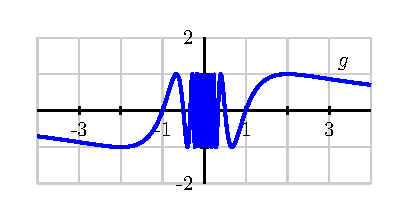
\includegraphics{figures/1_2_Ex1g.eps} 

\begin{example} \label{Ex:1.1.Eg2}
Use both tables and graphical approaches to investigate and, if possible, estimate or determine the value of the limit for the following function at the specified values. 
\[ \ds g(x) = \sin\left( \frac{\pi}{x} \right); \quad a = 3, \ a = 0\]

\solution Again, we construct two tables and a graph, see Table~\ref{T:1-1_Eg2} and Figure~\ref{fig:1-1_Eg2}.

First, as $x \to 3$, it appears from the data (and the graph) that the function is approaching approximately $0.866025$.  To be precise, we have to use the fact that $\frac{\pi}{x} \to \frac{\pi}{3}$, and thus we find that $g(x) = \sin(\frac{\pi}{x}) \to \sin(\frac{\pi}{3})$ as $x \to 3$.  The exact value of $\sin(\frac{\pi}{3})$ is $\frac{\sqrt{3}}{2}$, which is approximately 0.8660254038.  Thus, we see that
$$\lim_{x \to 3} g(x) = \frac{\sqrt{3}}{2}.$$

As $x \to 0$, we observe that $\frac{\pi}{x}$ does not behave in an elementary way.  When $x$ is positive and approaching zero, we are dividing by smaller and smaller positive values, and $\frac{\pi}{x}$ increases without bound.  When $x$ is negative and approaching zero, $\frac{\pi}{x}$ decreases without bound.  In this sense, as we get close to $x = 0$, the inputs to the sine function are growing rapidly, and this leads to wild oscillations in the graph of $g$.  It is an instructive exercise to plot the function $g(x) = \sin\left(\frac{\pi}{x}\right)$ with a graphing utility and then zoom in on $x = 0$.  Doing so shows that the function never settles down to a single value near the origin and suggests that $g$ does not have a limit at $x = 0$.
\end{example} % EXAMPLE

\begin{margintable}[6cm]
\begin{tabular}{c|c||c|c}
	$x$ & $f(x)$ & $x$ & $f(x)$ \\ \hline
	$0.5$ & $1.5$ & $1.5$ & \hspace{.75in} \\
	$0.9$ & \hspace{.75in} & $1.1$ & $2.1$ \\
	$0.99$ & $1.99$ & $1.01$ & \hspace{.75in} \\
	$0.999$ & \hspace{.75in} & $1.001$ & $2.001$ \\
\end{tabular}
\caption{Tabe of values near $x=1$.}
\label{T:1-1_Act1}
\end{margintable}

\begin{activity} \label{A:1.1.1}  Consider the function $f(x) = \dfrac{x^2 - 1}{x - 1}$.
\ba
\item Does the value of $f(1)$ exist? Why/why not?

\item Use a calculator or spreadsheet to fill in the blanks of Table~\ref{T:1-1_Act1}. Some of these have already been done for you; your calculations should not be drastically different from the ones already here. For example a calculation equal to 22.5 is very likely incorrect. Based on the table, estimate the value of $\ds \lim_{x \to 1} \frac{x^2 - 1}{x-1}$. 

\item Plot an accurate graph of the function $f$.  It should be a straight line.  Using your plot, what is $f(1)$?  What is $\ds \lim_{x \to 1} f(x)$?

\item Now use algebra to simplify the fraction $\dfrac{x^2 - 1}{x - 1}$. Call this new function $g(x)$.  What is $\ds \lim_{x \to 1} g(x)$? How is this limit related to the limit of $f(x)$ as $x$ approaches $1$?
\ea
\end{activity}

\aftera
 % ACTIVITY

An important lesson to take from Example~\ref{Ex:1.1.Eg2} is that both graphs and tables can be misleading when determining the value of a limit.  While a table of values is useful for investigating the possible value of a limit, we should also use other tools to confirm the value, if we think the table suggests the limit exists.

%-----------------------------------------------------------------------
% SUBSECTION IDENTIFYING WHEN LIMITS DO NOT EXIST
%-----------------------------------------------------------------------
\subsection{Identifying When Limits Do Not Exist}

As we have seen in Example~\ref{Ex:1.1.Eg2}, a function may not have a limit for all values of $x$. That is, we cannot say $\ds \lim_{x\to a}f(x)=L$ for some numbers $L$ for all values of $a$, for there may not be a number that $f(x)$ is approaching. There are three ways in which a limit may fail to exist. \index{limit!does not exist}
\begin{enumerate}[1)]
\item The function $f(x)$ may approach different values on either side of $a$.
\item The function may grow without upper or lower bound as $x$ approaches $a$.
\item The function may oscillate as $x$ approaches $a$, which we saw in Example~\ref{Ex:1.1.Eg2}.
\end{enumerate}

\begin{example} \label{Ex:1.1.Eg5}
Explore why $\ds \lim_{x\to 1} f(x)$ does not exist, where 
\[ f(x) = \left\{ \begin{array}{cl} x^2-2x+3 & x\leq 1 \\ x & x>1 \end{array} \right..\]

\solution A graph of $f(x)$ around $x=1$ is given in Figure~\ref{fig:1-1_Eg5}. It is clear that as $x$ approaches 1, $f(x)$ does not approach a single number. Instead, $f(x)$ approaches two different numbers. When considering values of $x$ less than 1 (approaching 1 from the left), $f(x)$ is approaching 2; when considering values of $x$ greater than 1 (approaching 1 from the right), $f(x)$ is approaching 1. Recognizing this behavior is important; we'll study this in greater depth later. Right now, it suffices to say that the limit does not exist since $f(x)$ is not approaching a single value as $x$ approaches 1.
\end{example}

\begin{marginfigure}[-8cm]
\margingraphics{figs/1/fignolimit1.pdf}
\caption{Observing no limit as $x\to 1$.}\label{fig:1-1_Eg5}
\end{marginfigure} % EXAMPLE

\begin{marginfigure}[1cm]
\margingraphics{figs/1/fignolimit2.pdf}
\caption{Observing no limit as $x \to 1$.}\label{fig:1-1_Eg6}
\end{marginfigure}

\begin{example} \label{Ex:1.1.Eg6}
Explore why $\ds \lim_{x\to 1} \frac{1}{(x-1)^2}$ does not exist.

\solution A graph of $\ds f(x) = \frac{1}{(x-1)^2}$ is given in Figure~\ref{fig:1-1_Eg6}. It shows that as $x$ approaches 1, $f(x)$ grows without bound in the positive direction. 

We can deduce this on our own, without the aid of the graph or table. If $x$ is near 1, then $(x-1)^2$ is very small, and: 
\[ \frac{1}{\text{very small number}} \rightarrow \text{very large number}.\]
Since $f(x)$ is not approaching a single number (growing without bound), we conclude that 
\[ \lim_{x \to 1} \frac{1}{(x-1)^2} \] 
does not exist.
\end{example} % EXAMPLE

%----------------------------------------------------------------------------
% SUBSECTION COMPUTING LIMITS
%----------------------------------------------------------------------------
\subsection{Computing Limits} 

Thus far, our method of finding a limit is making a really good approximation either graphically or numerically.  Later, we will cover the precise method of $\epsilon$--$\delta$ proofs\footnote{See Section~\ref{S:1.4.precise} for more on the precise definition of a limit.} which can be quite cumbersome. Now, we will cover a series of laws which allow us to find limits analytically. 

Suppose that $\ds \lim_{x\to 2} f(x)=2$ and $\ds \lim_{x\to 2} g(x) = 3$. What is \newline $\ds \lim_{x\to 2}(f(x)+g(x))$? Intuition tells us that the limit should be $5$, as we wish limits to behave in a nice way. The following concept states that already established limits do behave nicely.

\concept{Limit Laws}{\small % CONCEPT
Let $b$, $c$, $L$ and $K$ be real numbers, let $n$ be a positive integer, and let $f$ and $g$ be functions with the following limits: \index{limit!properties}
\[ \lim_{x \to c}f(x) = L \text{\ and\ } \lim_{x\to c} g(x) = K. \]
The following limits hold.
\begin{enumerate}[1)]
\item \parbox{80pt}{Constants:} $\ds \lim_{x\to c} b = b$
\item \parbox{80pt}{Identity: } $\ds \lim_{x\to c} x = c$
\item \parbox{80pt}{Sums/Differences:} $\ds \lim_{x\to c}(f(x)\pm g(x)) = L\pm K$
\item \parbox{80pt}{Scalar Multiples:}	$\ds \lim_{x\to c} b\cdot f(x) = bL$
\item \parbox{80pt}{Products:} $\ds \lim_{x\to c} f(x)\cdot g(x) = LK$
\item \parbox{80pt}{Quotients:} $\ds \lim_{x\to c} f(x)/g(x) = L/K$, ($K\neq 0)$
\item \parbox{80pt}{Powers:} 	$\ds \lim_{x\to c} f(x)^n = L^n$
\item \parbox{80pt}{Roots:} \parbox[t]{185pt}{$\ds \lim_{x\to c} \sqrt[n]{f(x)} = \sqrt[n]{L}$ \qquad \small (if $n$ is even then $L$ must be greater than $0$.)}
\item \parbox{80pt}{Compositions:} \parbox[t]{200pt}{Adjust our previously given limit situation to: 
\[ \lim_{x\to c}f(x) = L \text{\ and\ } \lim_{x\to L} g(x) = K.\] 
Then $\ds \lim_{x\to c}g(f(x)) = K$.}
\end{enumerate}
} % end concept

\begin{example} \label{Ex:1.1.Eg3}
Let $\ds \lim_{x\to 2} f(x)=2$, $\ds  \lim_{x\to 2} g(x) = 3$ and $\ds p(x) = 3x^2-5x+7$. Find the following limits:

\begin{enumerate}[1)]
\item $\ds \lim_{x\to 2} \big(f(x) + g(x)\big)$
\item $\ds \lim_{x\to 2} \big(5f(x) + g(x)^2\big)$
\item $\ds \lim_{x\to 2} p(x)$
\end{enumerate}

\solution

\begin{enumerate}[1)]
\item Using the Sum/Difference rule, we know that \newline $\ds \lim_{x\to 2} \big(f(x) + g(x)\big) = 2+3 =5$.
\item Using the Scalar Multiple, Sum/Difference, and Power rules, we find that $\ds \lim_{x\to 2} \big(5f(x) + g(x)^2\big) = 5\cdot 2 + 3^2 = 19.$
\item Here we combine the Power, Scalar Multiple, Sum/Difference and Constant Rules. We show quite a few steps, but in general these can be omitted:
\begin{align*}
\lim_{x\to 2} p(x) &= \lim_{x\to 2} (3x^2-5x+7) \\
&= \lim_{x\to 2} 3x^2-\lim_{x\to 2} 5x+\lim_{x\to 2}7 \\
&= 3\cdot 2^2 - 5\cdot 2+7 \\
&= 9
\end{align*}
\end{enumerate}
\end{example} %EXAMPLE

Notice that in the last part of the previous example, we have
\[ \lim_{x \to 2} p(x) = p(2) = 9,\]
meaning that we could have evaluated the limit simply by directly substituting the value of $a$ into the function.  That is possible because the function $p(x)$ is {\em continuous}\sidenote{See Section~\ref{S:1.3.Continuity} for more on the notion of continuity.}, which means that the limit of the function at any point is equal to its function value.

From Example~\ref{Ex:1.1.Eg1}, we can evaluate the limit $\ds \lim_{x \to -1} \frac{4-x^2}{x+2}$ by evaluating the function at $x = -1$:
\[ \lim_{x \to -1} \frac{4-x^2}{x+2} = \frac{4 - (-1)^2}{-1 + 2} = \frac{4-1}{1} = 3. \]
Or from Example~\ref{Ex:1.1.Eg2}, we can evaluate the limit $\ds \lim_{x \to 3} \sin \left( \frac{\pi}{x} \right)$ by evaluating the function at $x = 3$:
\[ \lim_{x \to 3} \sin \left( \frac{\pi}{x} \right) = \sin \left( \frac{\pi}{3} \right) = \frac{\sqrt{3}}{2}. \]
This method is quite important and is stated again for emphasis.

\concept{Direct Substitution} % CONCEPT
{If $f$ is a continuous function and $a$ is in the domain of $f$, then 
\[ \lim_{x \to a} f(x) = f(a) \] 
} %end concept

For $f(x)$ in Example~\ref{Ex:1.1.Eg1}, the situation is more complicated when $x \to -2$ since $f(-2)$ is not defined.  If we attempt to evaluate the limit using direct substitution, we observe that 
\[ \lim_{x \to -2} \frac{4-x^2}{x+2} = \frac{4 - (-2)^2}{-2 + 2} = \frac{4-4}{-2+2} = \frac{0}{0}. \]
We call $0/0$ an \emph{indeterminate form}\index{indeterminate}, or mathematical gibberish, and it tells us nothing about the limit---it could exist, it could not exist, we just don't know.  We simply observe that it tells us there is somehow more work to do.  From the table and graph of Example~\ref{Ex:1.1.Eg1}, it appears that $f$ should have a limit of $4$ at $x = -2$.  To see algebraically why this is the case, let's work directly with the form of $f(x)$.  Observe that
\begin{eqnarray*}
\lim_{x \to -2} f(x) & = & \lim_{x \to -2} \frac{4-x^2}{x+2} \\
& = & \lim_{x \to -2} \frac{(2-x)(2+x)}{x+2}. \\
\end{eqnarray*}
At this point, it is important to observe that since we are taking the limit as $x \to -2$, we are considering $x$ values that are close, but not equal, to $-2$.  Since we never actually allow $x$ to equal $-2$, the quotient $\frac{2+x}{x+2}$ has value 1 for every possible value of $x$.  Thus, we can simplify the most recent expression above, and now find that
\[ \lim_{x \to -2} \frac{4-x^2}{x+2} = \lim_{x \to -2} \frac{(2-x)(2+x)}{x+2} = \lim_{x \to -2} (2-x). \]
Because $2-x$ is simply a linear function, this limit is now easy to determine, and its value clearly is $4$.  Thus, from several points of view we've seen that $\ds\lim_{x \to -2} f(x) = 4.$

\input{activities/1.1.Act2} % ACTIVITY

The section could have been titled ``Using Known Limits to Find Unknown Limits.'' By knowing certain limits of functions, we can find limits involving sums, products, powers, etc., of these functions. We further the development of such comparative tools with the Squeeze Theorem, a clever and intuitive way to find the value of some limits. 

Suppose we have functions $f$, $g$ and $h$ where $g$ always takes on values between $f$ and $h$; that is, for all $x$ in an interval, 
\[ f(x) \leq g(x) \leq h(x). \] 
If $f$ and $h$ have the same limit at $c$, and $g$  is always ``squeezed'' between them, then $g$ must have the same limit as well. That is what the Squeeze Theorem states.

\concept{Squeeze Theorem} % CONCEPT
{Let $f$, $g$ and $h$ be functions on an open interval $I$ containing $c$ such that for all $x$ in $I$, $f(x)\leq g(x) \leq h(x)$. If 
\[ \lim_{x\to c} f(x) = L = \lim_{x\to c} h(x),\] 
then 
\[ \lim_{x\to c} g(x) = L.\] \index{limit!Squeeze Theorem}\index{Squeeze Theorem}
} % end concept

It can take some work to figure out appropriate functions by which to ``squeeze'' the given function you are trying to evaluate a limit of. However, that is generally the only place work is necessary; the theorem makes the ``evaluating the limit part'' very simple. %We use the Squeeze Theorem in the following example to prove that $\ds \lim_{x\to 0} \frac{\sin(x)}{x} = 1$.

\begin{example}\label{Ex:1.1.Eg9}
Given $4x-9 \leq f(x) \leq x^2-4x+7$, use the Squeeze Theorem to find $\ds \lim_{x \to 4} f(x)$.

\solution We begin by finding $\ds \lim_{x \to 4} (4x-9)$ and \newline $\ds \lim_{x \to 4} (x^2-4x+7)$. 
\[ \lim_{x \to 4} (4x-9) = 4(4)-9 = 7 \]
and 
\[ \lim_{x \to 4} (x^2-4x+7) = (4)^2-4(4)+7 = 7. \]
Therefore,
\[ \lim_{x \to 4} (4x-9) = 7 = \lim_{x \to 4} (x^2-4x+7),\]
and by the Squeeze Theorem, $\ds \lim_{x \to 4} f(x) = 7$.
\end{example} % EXAMPLE

\begin{activity}  \label{A:1.1.5}
In this activity, we prove $\ds \lim_{\theta \to 0} \frac{\sin(\theta)}{\theta} = 1$ using the squeeze theorem.  
\ba
	\item Draw the part of the unit circle that lies in the first quadrant. Place a point on the circle in the first quadrant and label it $(x,y)$.
	\item Draw the line connecting the origin to the point $(x,y)$ on the same graph. Label the angle between the line and the $x-axis$ as $\theta$.
	\item Find the area of the sector of the unit circle subtended by $\theta$ that you drew above.
	\item Draw a vertical line from the point $(x,y)$ to the $x$-axis. This will form a right triangle. \label{small}
	\item Find the area of the triangle in (\ref{small}) in terms of $\theta$. You will need to use trig functions. 
	\item Draw a line on the picture connecting the points $(1,0)$ and $(1,1)$. This will also form a right triangle. \label{large}
	\item Find the area of the triangle in (\ref{large}). You will need to use trig functions.
	\item What is the relationship between the three areas you found? Write this as an inequality.
	\item Write this inequality so that it involves the function $\frac{\sin(\theta)}{\theta}$.
	\item Now apply the squeeze theorem to get the result.
\ea
\end{activity}

%\begin{marginfigure}
%\margingraphics{figs/1/figSqueeze1.pdf}
%\caption{The unit circle and related triangles.}\label{fig:1-1_Eg4}
%\end{marginfigure}

\begin{activitySolution}
	We begin by considering the unit circle. Each point on the unit circle has coordinates $(\cos (\theta),\sin (\theta))$ for some angle $\theta$ as shown in Figure~\ref{fig:1-1_Eg4}. Using similar triangles, we can extend the line from the origin through the point to the point $(1,\tan (\theta))$, as shown. (Here we are assuming that $0 \leq \theta \leq \pi/2$. Later we will show that we can also consider $\theta \leq 0$.)

The area of the large triangle is $\frac{1}{2} \tan(\theta)$; the area of the sector is $\theta/2$; the area of the triangle contained inside the sector is $\frac{1}{2} \sin(\theta)$. It is then clear from the diagram that 
\[ \frac{\tan (\theta)}{2} \geq \frac{\theta}{2} \geq \frac{\sin (\theta)}{2}.\]

Multiply all terms by $\ds \frac{2}{\sin(\theta)}$, giving 
\[ \frac{1}{\cos(\theta)} \geq \frac{\theta}{\sin (\theta)} \geq 1.\]

Taking reciprocals reverses the inequalities, giving 
\[ \cos (\theta) \leq \frac{\sin(\theta)}{\theta} \leq 1.\]
These inequalities hold for all values of $\theta$ near 0, even negative values, since $\cos (-\theta) = \cos(\theta)$ and $\sin (-\theta) = -\sin (\theta)$.

Now take the limit of everything as $\theta \to 0$.

\[ \lim_{\theta \to 0} \cos (\theta) \leq \lim_{\theta \to 0} \frac{\sin(\theta)}{\theta} \leq \lim_{\theta \to 0}  1 \]
\[ \cos 0 \leq \lim_{\theta \to 0} \frac{\sin(\theta)}{\theta} \leq  1 \]
\[ 1 \leq \lim_{\theta \to 0} \frac{\sin(\theta)}{\theta} \leq  1 \]

By the Squeeze Theorem, $\ds \lim_{\theta \to 0} \frac{\sin(\theta)}{\theta}=1$.
\end{activitySolution}
\aftera
 % ACTIVITY

%------------------------------------------
% SUBSECTION ONE-SIDED LIMITS
%------------------------------------------
\subsection*{One-Sided Limits}

In this section, we explored the three ways in which limits of functions failed to exist: 
\begin{enumerate}[1)]
\item The function approached different values from the left and right,
\item The function grows without bound, and 
\item The function oscillates as $x$ approaches $a$.
\end{enumerate}
	
Now we explore in depth the concepts behind item \#1 by introducing the \textit{one-sided limit}. We begin with  definitions that are very similar to the definition of the limit given earlier, but the notation is slightly different.

\definition{One-Sided Limits}{ % DEFINTION
\textbf{Left-Sided Limit:} \index{limit!one sided}\index{limit!right sided}\index{limit!left sided} Let $f$ be a function defined on an open interval containing $a$. The notation 
\[ \lim_{x \to a^-} f(x) = L \] 
is read as ``the limit of $f(x)$ as $x$ approaches $a$ from the left is $L$,'' or ``the \textit{left-sided limit of $f$ at $a$ is L}''.\\

\noindent\textbf{Right-Sided Limit:} Let $f$ be a function defined on an open interval containing $a$. The notation 
\[ \lim_{x \to a^+} f(x) = L \] 
is read as ``the limit of $f(x)$ as $x$ approaches $a$ from the right is $L$,'' or ``the \textit{right-sided limit of $f$ at $a$ is L}''.
} % end definition

Practically speaking, when evaluating a left-hand limit, we consider only values of $x$ ``to the left of $a$,'' i.e., where $x<a$. The admittedly imperfect notation $x \to a^-$ is used to imply that we look at values of $x$ to the left of $a$. The notation has nothing to do with positive or negative values of either $x$ or $a$. 

A similar statement holds for evaluating right-hand limits; there we consider only values of $x$ to the right of $a$, i.e., $x>a$. We can use the Limit Laws given earlier to help us evaluate these limits; we just restrict our view to one side of $a$.

\begin{marginfigure}[8cm]
\margingraphics{figs/1/figOneSidedLimits1.pdf}
\caption{The graph of $f$.}\label{fig:1-1_Eg7}
\end{marginfigure}

%\mfigure{.7}{A graph of $f$ in Example \ref{ex_onesidea}.}{fig:onesided1}{figures/figOneSidedLimits1}}

\begin{example} \label{Ex:1.1.Eg7}
Let $\ds f(x) = \left\{\begin{array}{cc} x & 0\leq x\leq 1 \\ 3-x & 1<x<2\end{array},\right.$ as shown in Figure~\ref{fig:1-1_Eg7}. Find each of the following: 
\begin{multicols}{2}
\begin{enumerate}[1)]
\item		$\ds \lim_{x\to 1^-} f(x)$
\item		$\ds \lim_{x\to 1^+} f(x)$
\item		$\ds \lim_{x\to 1} f(x)$
\item		$\ds f(1)$
\item		$\ds \lim_{x\to 0^+} f(x)$
\item		$f(0)$
\item		$\ds \lim_{x\to 2^-} f(x)$
\item		$f(2)$
\end{enumerate}
\end{multicols}

\solution For these problems, the visual aid of the graph is likely more effective in evaluating the limits than using $f$ itself. Therefore we will refer often to the graph.
\begin{enumerate}[1)]
\item As $x$ goes to $1$ \textit{from the left}, we see that $f(x)$ is approaching the value of $1$. Therefore $\ds \lim_{x\to 1^-} f(x) =1.$

\item As $x$ goes to $1$ \textit{from the right}, we see that $f(x)$ is approaching the value of $2$. Recall that it does not matter that there is an ``open circle'' there; we are evaluating a limit, not the value of the function. Therefore $\ds \lim_{x\to 1^+} f(x)=2$.

\item The limit of $f$ as $x$ approaches $1$ does not exist, as discussed earlier. The function does not approach one particular value, but two different values from the left and the right.

\item Using the definition and by looking at the graph we see that $f(1) = 1$.

\item As $x$ goes to $0$ from the right, we see that $f(x)$ is also approaching $0$. Therefore $\ds \lim_{x\to 0^+} f(x)=0$. Note we cannot consider a left-hand limit at $0$ as $f$ is not defined for values of $x<0$.

\item Using the definition and the graph, $f(0) = 0$.

\item As $x$ goes to $2$ from the left, we see that $f(x)$ is approaching the value of $1$. Therefore $\ds \lim_{x\to 2^-} f(x)=1.$

\item The graph and the definition of the function show that $f(2)$ is not defined.
\end{enumerate}
\end{example}


 % EXAMPLE

Note how the left and right-hand limits were different; this, of course, causes the two-sided limit to not exist. The following theorem states what is fairly intuitive: the two-sided limit exists precisely when the left and right-hand limits are equal.

\concept{Limits and One Sided Limits} % CONCEPT
{Let $f$ be a function defined on an open interval $I$ containing $a$. \index{limit!does not exist} Then 
\[ \lim_{x \to a}f(x) = L\] 
if, and only if, 
\[ \lim_{x \to a^-}f(x) = L \quad \text{and} \quad \lim_{x \to a^+}f(x) = L.\]
} % end concept

The phrase ``if, and only if'' means the two statements are \textit{equivalent}: they are either both true or both false. If the limit equals $L$, then the left and right hand limits both equal $L$. If the limit is not equal to $L$, then at least one of the left and right-hand limits is not equal to $L$ (it may not even exist).

One thing to consider is that the value of the function may/may not be equal to the value(s) of its left/right-hand limits, even when these limits agree.

\begin{marginfigure}[8cm]
\margingraphics{figs/1/figOneSidedLimits3.pdf}
\caption{The graph of $f$.}\label{fig:1-1_Eg8}
\end{marginfigure}

\begin{example} \label{Ex:1.1.Eg8}
Let $f(x) = \left\{\begin{array}{cc} (x-1)^2 & 0\leq x\leq 2, x\neq 1\\ 1 & x=1\end{array},\right.$ as shown in Figure~\ref{fig:1-1_Eg8}. Evaluate the following.
\begin{multicols}{2}
\begin{enumerate}[1)]
\item $\ds \lim_{x\to 1^-} f(x)$
\item $\ds \lim_{x\to 1^+} f(x)$
\item $\ds \lim_{x\to 1} f(x)$
\item $f(1)$
\end{enumerate}
\end{multicols}

\solution It is clear by looking at the graph that both the left and right-hand limits of $f$, as $x$ approaches $1$, is $0$. Thus it is also clear that the limit is $0$; i.e., $\ds \lim_{x\to 1} f(x) = 0$. It is also clearly stated that $f(1) = 1$.
\end{example} % EXAMPLE

This concludes a rather lengthy introduction to the notion of limits.  It is important to remember that our primary motivation for considering limits of functions comes from our interest in studying the rate of change of a function.  To that end, we close this section by revisiting our previous work with average and instantaneous velocity and highlighting the role that limits play. 

%-----------------------------------------------------
% SUBSECTION INSTANTANEOUS VELOCITY
%-----------------------------------------------------
\subsection*{Instantaneous Velocity}

Suppose that we have a moving object whose position at time $t$ is given by a function $s$.  We know that the average velocity of the object on the time interval $[a,b]$ is $AV_{[a,b]} = \frac{s(b)-s(a)}{b-a}.$  We define the \emph{instantaneous velocity} \index{instantaneous velocity} at $a$ to be the limit of average velocity as $b$ approaches $a$.  Note particularly that as $b \to a$, the length of the time interval gets shorter and shorter (while always including $a$).  In Section~\ref{S:2.1.DerivativePt}, we will introduce a helpful shorthand notation to represent the instantaneous rate of change.  For now, we will write $IV_{t=a}$ for the instantaneous velocity at $t = a$, and thus
$$IV_{t=a} = \lim_{b \to a} AV_{[a,b]} = \lim_{b \to a} \frac{s(b)-s(a)}{b-a}.$$
Equivalently, if we think of the changing value $b$ as being of the form $b = a + h$, where $h$ is some small number, then we may instead write
$$IV_{t=a} = \lim_{h \to 0} AV_{[a,a+h]} = \lim_{h \to 0} \frac{s(a+h)-s(a)}{h}.$$
Again, the most important idea here is that to compute instantaneous velocity\index{instantaneous velocity}, we take a limit of average velocities as the time interval shrinks.  Two different activities offer the opportunity to investigate these ideas and the role of limits further. \\

\input{activities/1.1.Act3} % ACTIVITY

The closing activity of this section asks you to make some connections among average velocity, instantaneous velocity, and slopes of certain lines.
\newpage
\input{activities/1.1.Act4} % ACTIVITY

%\begin{authornote}
%This is an author note.
%\end{authornote}

%--------------
% SUMMARY
%--------------
\begin{summary}
\item Limits enable us to examine trends in function behavior near a specific point.  In particular, taking a limit at a given point asks if the function values nearby tend to approach a particular fixed value.

\item When we write $\ds \lim_{x \to a} f(x) = L$, we read this as saying ``the limit of $f$ as $x$ approaches $a$ is $L$,'' and this means that we can make the value of $f(x)$ as close to $L$ as we want by taking $x$ sufficiently close (but not equal) to $a$.

\item If we desire to know $\ds \lim_{x \to a} f(x)$ for a given value of $a$ and a known function $f$, we can estimate this value from the graph of $f$ or by generating a table of function values that result from a sequence of $x$-values that are closer and closer to $a$.  If we want the exact value of the limit, we need to work with the function algebraically and see if we can use familiar properties of known, basic functions to understand how different parts of the formula for $f$ change as $x \to a$. 

\item The instantaneous velocity of a moving object at a fixed time is found by taking the limit of average velocities of the object over shorter and shorter time intervals that all contain the time of interest.
\end{summary}

\clearpage

%--------------
% EXERCISES
%--------------
\begin{adjustwidth*}{}{-2.25in}
\textbf{{\large Exercises}}
\setlength{\columnsep}{25pt}
\begin{multicols*}{2}
\noindent Terms and Concepts \small

\begin{enumerate}[1)]
\item In your own words, what does it mean to ``find the limit of $f(x)$ as $x$ approaches 3''?
\item An expression of the form $\frac00$ is called \underline{\hskip 15pt}.
\item T/F: The limit of $f(x)$ as $x$ approaches $5$ is always $f(5)$.
\item T/F: If $\ds \lim_{x\to 1^-} f(x) = 5$, then $\ds \lim_{x\to 1} f(x) = 5$.
\item T/F: If $\ds \lim_{x\to 1^-} f(x) = 5$, then $\ds \lim_{x\to 1^+} f(x) = 5$.
\item T/F: If $\ds \lim_{x\to 1} f(x) = 5$, then $\ds \lim_{x\to 1^-} f(x) = 5$.
\item Describe three situations where $\displaystyle \lim_{x\to c}f(x)$ does not exist.
\end{enumerate} 

\noindent {\normalsize Problems\\} \small

\noindent In the following exercises, evaluate each expression using the given graph of $f(x)$.

\begin{enumerate}[1),resume]
\item 
\begin{minipage}{\linewidth}\centering
\includegraphics[scale=.8]{figures/fig01_04_ex_05}
\end{minipage}

\noindent\begin{minipage}[t]{.5\linewidth}
\begin{enumerate}
\item		$\ds \lim_{x\to 1^-} f(x)$
\item		$\ds \lim_{x\to 1^+} f(x)$
\item		$\ds \lim_{x\to 1} f(x)$
\end{enumerate}
\end{minipage}
\noindent\begin{minipage}[t]{.5\linewidth}
\begin{enumerate}\addtocounter{enumii}{3}
\item		$f(1)$
\item		$\ds \lim_{x\to 0^-} f(x)$
\item		$\ds \lim_{x\to 0^+} f(x)$
\end{enumerate}
\end{minipage}

\item
\begin{minipage}{\linewidth}\centering
\includegraphics[scale=.8]{figures/fig01_04_ex_06}
\end{minipage}

\noindent\begin{minipage}[t]{.5\linewidth}
\begin{enumerate}
\item		$\ds \lim_{x\to 1^-} f(x)$
\item		$\ds \lim_{x\to 1^+} f(x)$
\item		$\ds \lim_{x\to 1} f(x)$
\end{enumerate}
\end{minipage}
\noindent\begin{minipage}[t]{.5\linewidth}
\begin{enumerate}\addtocounter{enumii}{3}
\item		$f(1)$
\item		$\ds \lim_{x\to 2^-} f(x)$
\item		$\ds \lim_{x\to 2^+} f(x)$
\end{enumerate}
\end{minipage}

\item
\begin{minipage}{\linewidth}\centering
\includegraphics[scale=.8]{figures/fig01_04_ex_08}
\end{minipage}

\noindent\begin{minipage}[t]{.5\linewidth}
\begin{enumerate}
\item		$\ds \lim_{x\to 1^-} f(x)$
\item		$\ds \lim_{x\to 1^+} f(x)$
\end{enumerate}
\end{minipage}
\noindent\begin{minipage}[t]{.5\linewidth}
\begin{enumerate}\addtocounter{enumii}{2}
\item		$\ds \lim_{x\to 1} f(x)$
\item		$f(1)$
%\item		$\ds \lim_{x\to 2^-} f(x)$
%\item		$\ds \lim_{x\to 0^+} f(x)$
\end{enumerate}
\end{minipage}

\end{enumerate}

\vspace{.5cm}

\noindent Using:

\begin{tabular}{lll}
$\ds \lim_{x \to 9}f(x) = 6$ & \quad\quad &$\ds \lim_{x \to 6} f(x) = 9$\\
$\ds \lim_{x \to 9}g(x) = 3$ &  & $\ds \lim_{x \to 6} g(x) = 3$
\end{tabular}

\noindent evaluate the limits given in the following exercises, where possible. If it is not possible to know, state so.
\begin{enumerate}[1),resume]
\item $\ds \lim_{x\to9}(f(x)+g(x))$
\item $\ds \lim_{x\to9}(3f(x)/g(x))$
\item $\ds \lim_{x\to9}\left(\frac{f(x)-2g(x)}{g(x)}\right)$
\item $\ds \lim_{x\to6}\left(\frac{f(x)}{3-g(x)}\right)$
\item $\ds \lim_{x\to9}g\big(f(x)\big)$
\item $\ds \lim_{x\to6}f\big(g(x)\big)$
\item $\ds \lim_{x\to6}g\big(f(f(x))\big)$
\item $\ds \lim_{x\to6}f(x)g(x)-f\,^2(x)+g^2(x)$
\end{enumerate}

\vspace{.5cm}

\noindent Using:

\begin{tabular}{lll}
$\ds \lim_{x\to1}f(x) = 2$ & \quad\quad &$\ds \lim_{x\to10} f(x) = 1$\\
$\ds \lim_{x\to1}g(x) = 0$ &  & $\ds \lim_{x\to10} g(x) = \pi$
\end{tabular}

\noindent evaluate the limits given in the following exercises, where possible. If it is not possible to know, state so.
\begin{multicols}{2}
\begin{enumerate}[1),resume]
\item $\ds \lim_{x\to1}f(x)^{g(x)}$
\item $\ds \lim_{x\to10}\cos \big(g(x)\big)$
\item $\ds \lim_{x\to1}f(x)g(x)$
\item {$\ds \lim_{x\to1}g\big(5f(x)\big)$}
\end{enumerate}
\end{multicols}

\vspace{.5cm}

\noindent In the following exercises, evaluate the limit.
\begin{multicols}{2}
\begin{enumerate}[1),start=23]
\item {$\ds \lim_{x\to3}x^2-3x+7$}
\item {$\ds \lim_{x\to\pi}\frac{3x+1}{1-x}$}
\item {$\ds \lim_{x\to\pi}\frac{x^2+3x+5}{5x^2-2x-3}$}
\item {$\ds \lim_{x\to\pi}\left(\frac{x-3}{x-5}\right)^7$}
\item {$\ds \lim_{x\to\pi/4}\cos x\sin x$}
\item {$\ds \lim_{x\to0}\ln x$}
\end{enumerate}
\end{multicols}

%------------------------------------------
% END OF EXERCISES ON FIRST PAGE
%------------------------------------------
\end{multicols*}
\end{adjustwidth*}

\clearpage

\begin{adjustwidth*}{}{-2.25in}
\setlength{\columnsep}{25pt}
\begin{multicols*}{2}\small

\begin{multicols}{2}
\begin{enumerate}[1),start=29]
\item {$\ds \lim_{x\to3}4^{x^3-8x}$}
\item {$\ds \lim_{x\to\pi/6} \csc x$}
\item {$\ds \lim_{x\to0} \ln(1+x)$}
\item {$\ds \lim_{x\to6^-} \frac{x^2-4 x-12}{x^2-13 x+42}$}
\item {$\ds \lim_{x\to0^+} \frac{x^2+2 x}{x^2-2 x}$}
\item {$\ds \lim_{x\to2^-} \frac{x^2+6 x-16}{x^2-3 x+2}$}
\item {$\ds \lim_{x\to2^+}\frac{x^2-10 x+16}{x^2-x-2}$}
\item {$\ds \lim_{x\to-2}\frac{x^2-5 x-14}{x^2+10 x+16}$}
\item {$\ds \lim_{x\to-1}\frac{x^2+9 x+8}{x^2-6 x-7}$}
\item $\ds \lim_{x \to 1} \frac{x-1}{\sqrt{x} - 1}$
\item $\ds \lim_{x \to 0} \frac{\sqrt{x+4} - 2}{x}$
\item $\ds \lim_{x \to 0} \frac{\sqrt{16 + x} - 4}{x}$
\end{enumerate}
\end{multicols}

\vspace{.5cm}

\noindent Use the Squeeze Theorem, where appropriate, to evaluate the following limits.
\begin{enumerate}[1),start=41]
\item {$\ds \lim_{x \to 0} x \sin\left( \frac{1}{x} \right)$}
\item {$\ds \lim_{x\to0} \sin x\cos\left(\frac{1}{x^2}\right)$}
\item {$\ds \lim_{x\to3} f(x)$, where $x^2\leq f(x) \leq 3x$ on $[0,3]$.}
\end{enumerate}

\vspace{.5cm}

\noindent Using the techniques you learned in Activity~\ref{A:1.1.3} and Activity~\ref{A:1.1.4}, determine the instantaneous velocity of some object with given position function and specific instant.
\begin{enumerate}[1),start=44]
\item $\ds s(t) = -7t + 2; \quad t=3$
\item $\ds s(t) = 9t + 0.06; \quad t=1$
\item $\ds s(t) = t^2 + 3t - 7; \quad t=1$
\item $\ds s(t) = \frac{1}{t+1}; \quad t=2$
\end{enumerate}

%---------------------------------------------
% END OF EXERCISES ON SECOND PAGE
%---------------------------------------------
\end{multicols*}
\end{adjustwidth*}
\afterexercises 

\cleardoublepage
